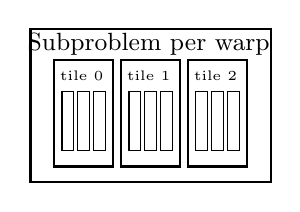
\begin{tikzpicture}[every node/.style={thick,rectangle,inner sep=0pt}]

\def \dx {0.05}
\def \dy {0.2}
\def \recx {0.15}
\def \recX {3*\recx + 4*\dx}
\def \recXX {3 * \recX + 22 * \dx}
\def \recy {0.75}
\def \recY {\recy + 3 * \dy}
\def \recYY {\recY + 3 * \dy}

%% left child 
\draw [black] (0 + 0, 0 + 0) rectangle (0 + \recx, 0 + \recy);
\draw [black] (0 + \recx + \dx, 0) rectangle (0 + 2*\recx + \dx, 0 + \recy);
\draw [black] (0 + 2*\recx + 2*\dx, 0 + 0) rectangle (0 + 3*\recx + 2*\dx, 0 + \recy);

\draw[thick, black] (0-2*\dx, 0-\dy) rectangle (0-2*\dx + \recX + 2 * \dx, 0-\dy + \recY);
\node () at (0 + 1 * \recx + 2 * \dx, \recy + \dy) {\tiny tile 0};

\draw [black] (\recX + 4*\dx + 0, 0 + 0) rectangle (\recX + 4*\dx + \recx, 0 + \recy);
\draw [black] (\recX + 4*\dx + \recx + \dx, 0) rectangle (\recX + 4*\dx + 2*\recx + \dx, 0 + \recy);
\draw [black] (\recX + 4*\dx + 2*\recx + 2*\dx, 0 + 0) rectangle (\recX + 4*\dx + 3*\recx + 2*\dx, 0 + \recy);

\draw[thick, black] (\recX + 4*\dx-2*\dx, 0-\dy) rectangle (\recX + 4*\dx-2*\dx + \recX + 2 * \dx, 0-\dy + \recY);
\node () at (\recX + 4*\dx + 1 * \recx + 2 * \dx, \recy + \dy) {\tiny tile 1};

\draw [black] (2*\recX + 12*\dx + 0, 0 + 0) rectangle (2*\recX + 12*\dx + \recx, 0 + \recy);
\draw [black] (2*\recX + 12*\dx + \recx + \dx, 0) rectangle (2*\recX + 12*\dx + 2*\recx + \dx, 0 + \recy);
\draw [black] (2*\recX + 12*\dx + 2*\recx + 2*\dx, 0 + 0) rectangle (2*\recX + 12*\dx + 3*\recx + 2*\dx, 0 + \recy);

\draw[thick, black] (2*\recX + 12*\dx-2*\dx, 0-\dy) rectangle (2*\recX + 12*\dx-2*\dx + \recX + 2 * \dx, 0-\dy + \recY);
\node () at (2*\recX + 12*\dx + 1 * \recx + 2 * \dx, \recy + \dy) {\tiny tile 2};

\draw [thick, black] (0-8*\dx, 0-2*\dy) rectangle (0 + \recXX, 0-2*\dy + \recYY);
\node () at (\recX + 4*\dx + 1 * \recx + 2 * \dx, \recy + 3* \dy) {\small Subproblem per warp};

% \def\dx{1}
% \def\a{0}
% \def\recx{0.15}
% \def\recy{0.75}
% \def \recyTile{2*\recy}
% \def \recxTile{5*\recx}
% \def \recxSubp{4 * \recxTile}
% \def \recySubp{1.5 * \recyTile}

% \node (a1) at (0 * \dx,0) [draw, minimum width=\recx cm, minimum height=\recy cm, anchor=north] {};
% \node (a2) [right=2pt of a1, draw=black,rectangle,minimum width = \recx cm, minimum height=\recy cm] {};
% \node (a3) [right=2pt of a2, draw=black,rectangle,minimum width = \recx cm, minimum height=\recy cm] {};
% \node (t1) [above=1pt of a2, anchor=south] {};

% \node (b1) [draw, fit=(a1)(a2)(a3)(t1), label={\scriptsize tile 0}, minimum width = \recxTile cm, minimum height=\recyTile cm] {};

% \node (a4) at (1 * \dx,0) [draw, minimum width=\recx cm, minimum height=\recy cm, anchor=north] {};
% \node (a5) [right=2pt of a4, draw=black,rectangle,minimum width = \recx cm, minimum height=\recy cm] {};
% \node (a6) [right=2pt of a5, draw=black,rectangle,minimum width = \recx cm, minimum height=\recy cm] {};
% \node (t4) [above=1pt of a5, anchor=south] {};

% \node (b4) [draw, fit=(a4)(a5)(a6)(t4), label={\scriptsize tile 1}, minimum width = \recxTile cm, minimum height=\recyTile cm] {};

% \node (a7) at (2 * \dx,0) [draw, minimum width=\recx cm, minimum height=\recy cm, anchor=north] {};
% \node (a8) [right=2pt of a7, draw=black,rectangle,minimum width = \recx cm, minimum height=\recy cm] {};
% \node (a9) [right=2pt of a8, draw=black,rectangle,minimum width = \recx cm, minimum height=\recy cm] {};
% \node (t7) [above=1pt of a8, anchor=south] {};

% \node (b7) [draw, fit=(a7)(a8)(a9)(t7), label={\scriptsize tile 2}, minimum width = \recxTile cm, minimum height=\recyTile cm] {};

% \node (c1) [draw, fit=(b7)(b4)(b1), label={\small Subproblem per warp}, minimum width = \recxSubp cm, minimum height=\recySubp cm] {};
\end{tikzpicture}